\newprob{1719147068}
{
    % act physcs p255 q14
    一個有500匝線圈的長螺線管連接至一個電路, 螺線管兩端為X 和Y。線圖顯示磁場B沿螺線管 中軸的變化。
    \par{\par\centering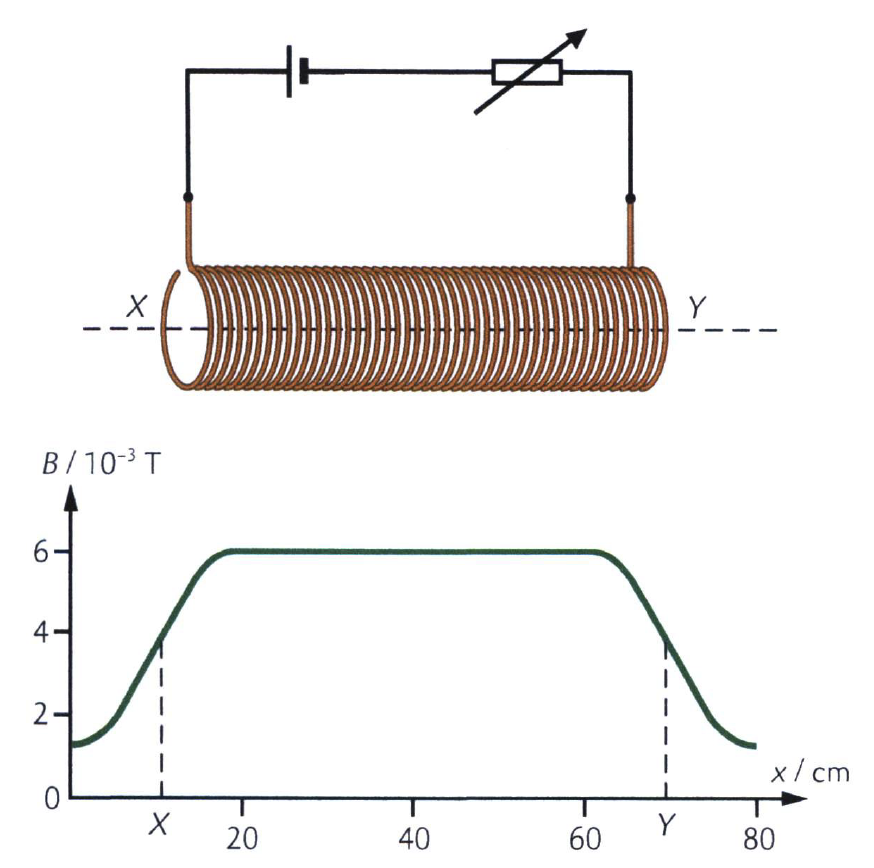
\includegraphics[width=.4\textwidth]{./img/ch4_magnetostatics_lq_2024-06-23-21-10-45.png}\par}
    \begin{parts}
        \part 試舉出一個合適的裝置,量度這個螺線管產 生的磁場。 \zzh{1}
        \part 線圖中的正數代表哪一個方向?\zzh{1}
        \part 通過螺線管的電流為多少? \zzh{3}
        \part 試舉出\textbf{兩個}方法,增強螺線管中的磁場。\zzh{2}
    \end{parts}
}{
    \par{\par\centering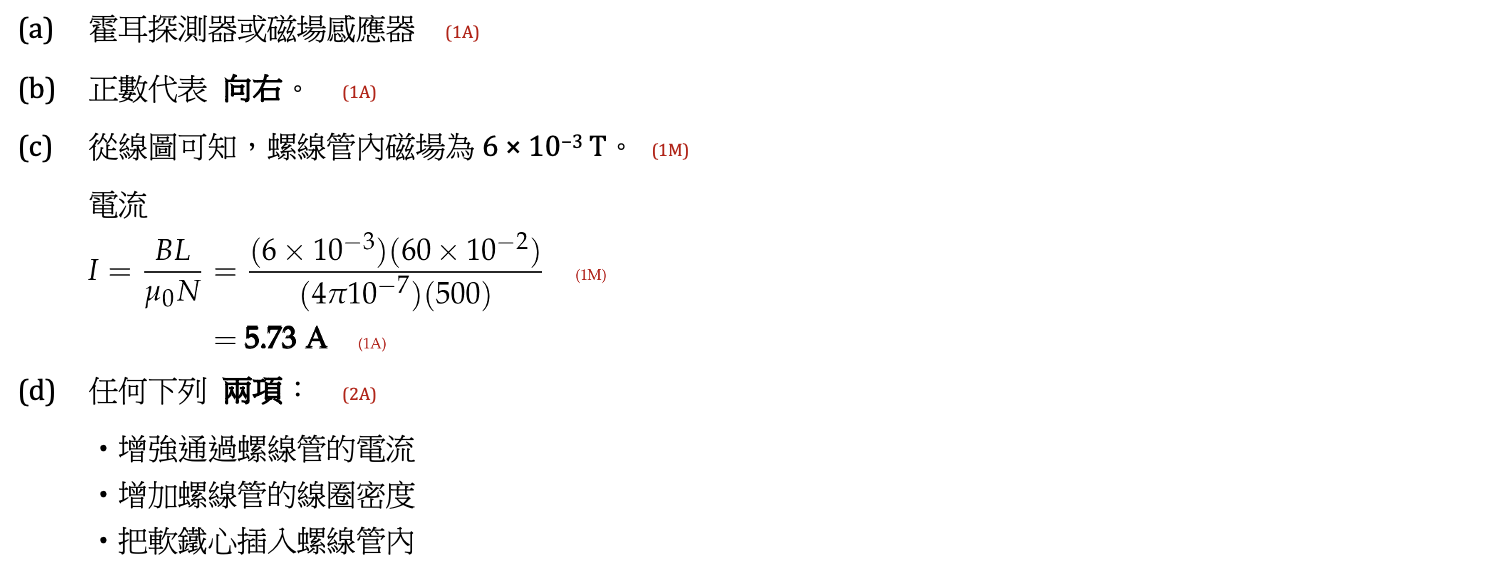
\includegraphics[width=\textwidth]{./img/ch4_magnetostatics_lq_2024-06-23-21-18-04.png}\par}
}

\newprob{1719148318}
{
    % act physcs p255 q15
    你現在獲得以下的儀器。試描述一個方法,探究 電磁鐵強度與線圈匝數的關係。 \zzh{6}
    \par{\par\centering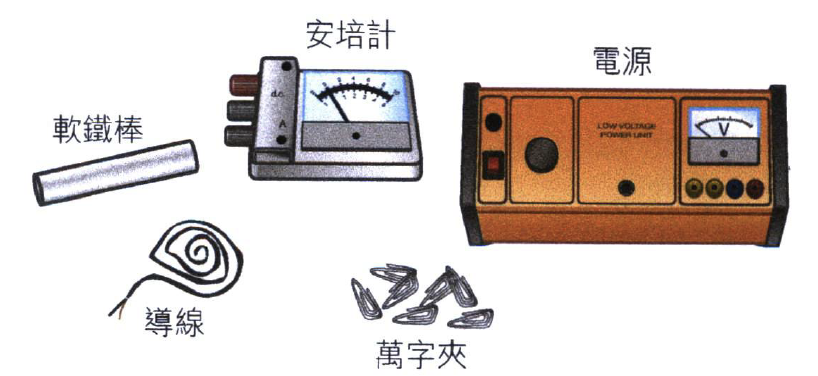
\includegraphics[width=.5\textwidth]{./img/ch4_magnetostatics_lq_2024-06-23-21-12-36.png}\par}
}{\par{\par\centering
\includegraphics[width=\textwidth]{./img/ch4_magnetostatics_lq_2024-06-23-21-18-19.png}\par}}

\newprob{1719148399}
{
    % act physcs p255 q16
    以下為一個簡單斷路器的示意圖。
    \par{\par\centering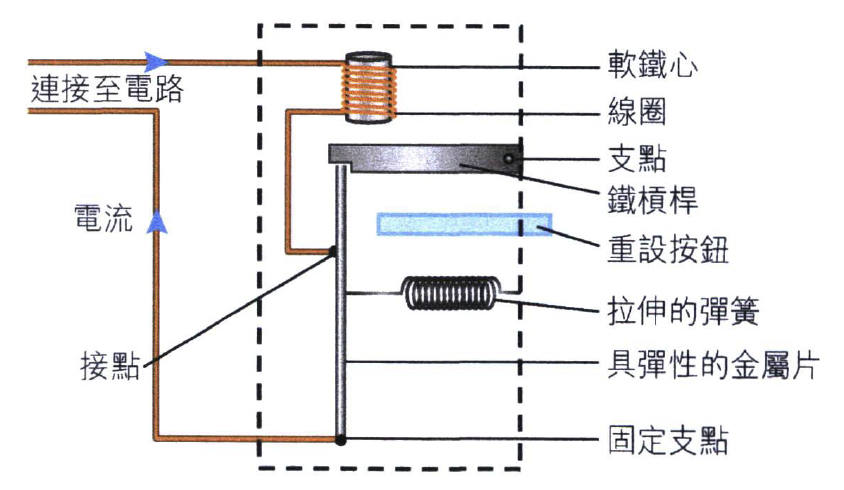
\includegraphics[width=.5\textwidth]{./img/ch4_magnetostatics_lq_2024-06-23-21-13-29.png}\par}
    \begin{parts}
        \part 一個很大的電流通過時,電路便會斷開,為 甚麼?\zzh{3}
        \part 故障修復後,應如何重設斷路器?試扼要解 釋。\zzh{2}
        \part 現在,斷路器通以一個正常大小的電流,電 路會再次斷開嗎?試扼要解釋。\zzh{2}
    \end{parts}
}{\par{\par\centering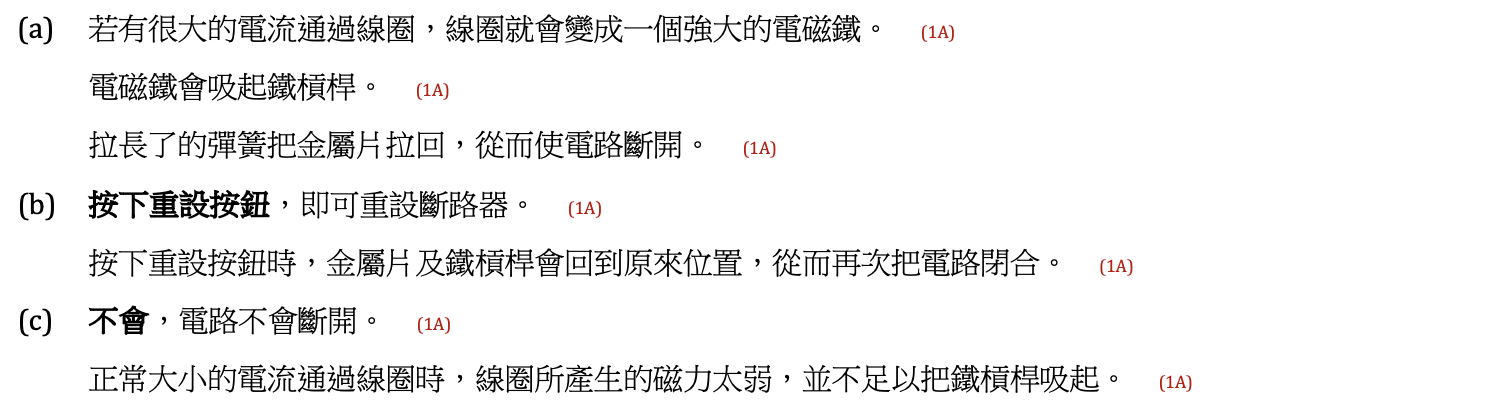
\includegraphics[width=\textwidth]{./img/ch4_magnetostatics_lq_2024-06-23-21-18-33.png}\par}}

\newprob{1719148447}
{
    % act physics p255 q17
    一個細小的長方形線圈放在一塊大磁鐵的兩極之 間,如圖。
    \par{\par\centering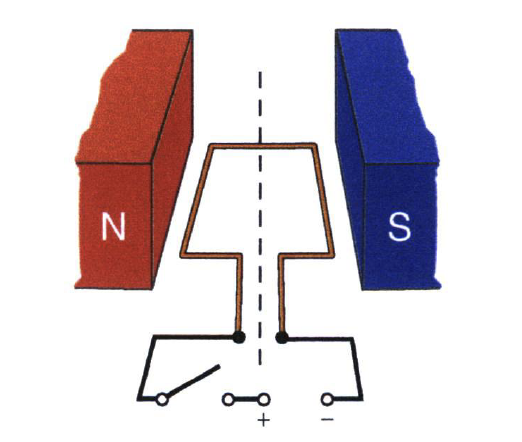
\includegraphics[width=.35\textwidth]{./img/ch4_magnetostatics_lq_2024-06-23-21-14-25.png}\par}
    \begin{parts}
        \part 當線圈受到最大的力矩,其平面與磁場應為 平行還是垂直? \zzh{1}
        \part 合上開關後,線圈繞垂直位置振盪數次,最 終停下。試扼要解釋其運動。\zzh{4}
        \part 有一個裝置能令電動機的線圈沿一個方向持 續旋轉。試寫出這裝置的名稱。\zzh{1}
    \end{parts}
}{\par{\par\centering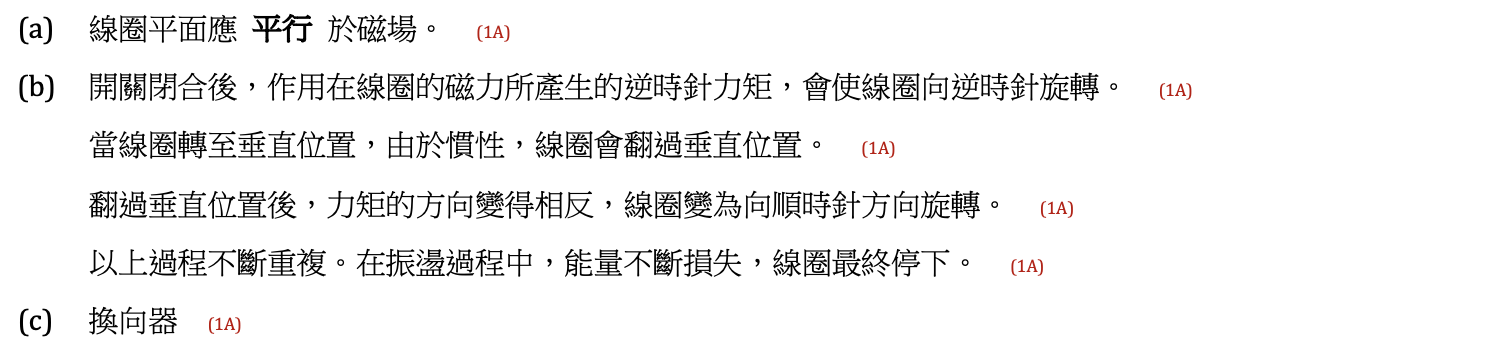
\includegraphics[width=\textwidth]{./img/ch4_magnetostatics_lq_2024-06-23-21-18-46.png}\par}}